\documentclass{article}
% \usepackage{xeCJK}
\usepackage{amsmath}
\usepackage{amssymb}
\usepackage{mathrsfs}
\usepackage{xcolor}
\usepackage{bm}
\usepackage{hyperref}
\usepackage{graphicx}
\usepackage{subcaption}
\usepackage{float}
\usepackage{multicol}
\usepackage{pdfpages}
\usepackage[ruled,linesnumbered]{algorithm2e}

\bibliographystyle{plain}
\setlength{\parindent}{2em}
\usepackage{geometry}
\geometry{a4paper, left=2.54cm, right=2.54cm, top=3.18cm, bottom=3.18cm}

% 设置文章行距
% \renewcommand{\baselinestretch}{1.5}

% define reference format
\hypersetup{
    colorlinks=true,
    linkcolor=blue,
    urlcolor=blue,
    citecolor=blue,
    linkbordercolor=white
}

\title{\textbf{Heterogeneous Frequency-Induced Synchronous Respiration in Frustrated Vicsek-Kuramoto Systems}}
\author{Yichen Lu}

\begin{document}

\maketitle

\tableofcontents

\section{The Model}

Particles are described by position $\mathbf{r}_i=\left( x_i, y_i \right)$ and phase angle $\theta_i$, evolving as:
\begin{subequations} 
    \label{eq:totalDynamicsMeanField}
    \begin{align}
        \dot{\mathbf{r}}_i&=v\mathbf{p}\left( \theta _i \right)+\sqrt{2D}\bm{\xi}_i\;\label{eq:dotR},
        \\
        \dot{\theta}_i&=\omega_i+\frac{K}{\left| A_i \right|}\sum_{j\in A_i}{F\left( \theta _j-\theta _i \right) }+\sqrt{2D_r}\eta _i\;\label{eq:dotTheta},
    \end{align}
\end{subequations}
for $i=1,2,\ldots,N$, where $N$ is the population size, $v$ is self-propulsion speed, $\mathbf{p}\left( \theta _i \right) =\left( \cos \theta _i,\sin \theta _i \right)$ is the unit vector in the orientation $\theta_i$, $\omega_i$ is the intrinsic frequency, $A_i\left( t \right) =\left\{ j: \left| \mathbf{r}_i\left( t \right) -\mathbf{r}_j\left( t \right) \right|\leqslant d_0 \right\}$ is the set of neighbors within coupling radius $d_0$ and $|A_i|$ is its cardinality, $K \left(\geqslant 0\right)$ is coupling strength, $\bm{\xi}$ and $\eta$ are Gaussian white noises with zero mean and unit variance, and $D$ and $D_r$ are translational and rotational diffusion coefficients, respectively. 
Here, the interaction function is defined as $F\left( \theta \right) =\sin \left( \theta +\alpha \right) -\sin \alpha $, where $\alpha$ is frustration.
The term $-\sin\alpha$ ensures synchronization ($\theta_j = \theta_i$) remains an equilibrium \cite{10.1143/PTP.79.1069}. 
This system generalizes alignments \cite{PhysRevLett.119.058002,PhysRevResearch.1.023026,Escaff2020,PhysRevLett.127.238001,PhysRevLett.133.258302}, anti-alignments \cite{PhysRevE.109.024602,PhysRevE.110.024603}, and self-propelled chimera \cite{PhysRevE.98.032219,PhysRevE.102.022604}. It reduces to normal Vicsek–Kuramoto for $\alpha=0$ and anti-aligning interactions for $\alpha=\pi$.
We set $\omega_i=0$ (identical particles) for simplifying the theoretical analysis and $D=D_r=0$ (deterministic dynamics) for clarity; simulations with heterogeneous frequencies and noise are provided in the Supplemental Material \cite{mycomment2023}, which manifest qualitatively similar behaviors.


\section{Behaviors}

\begin{figure}[H]
    \centering
    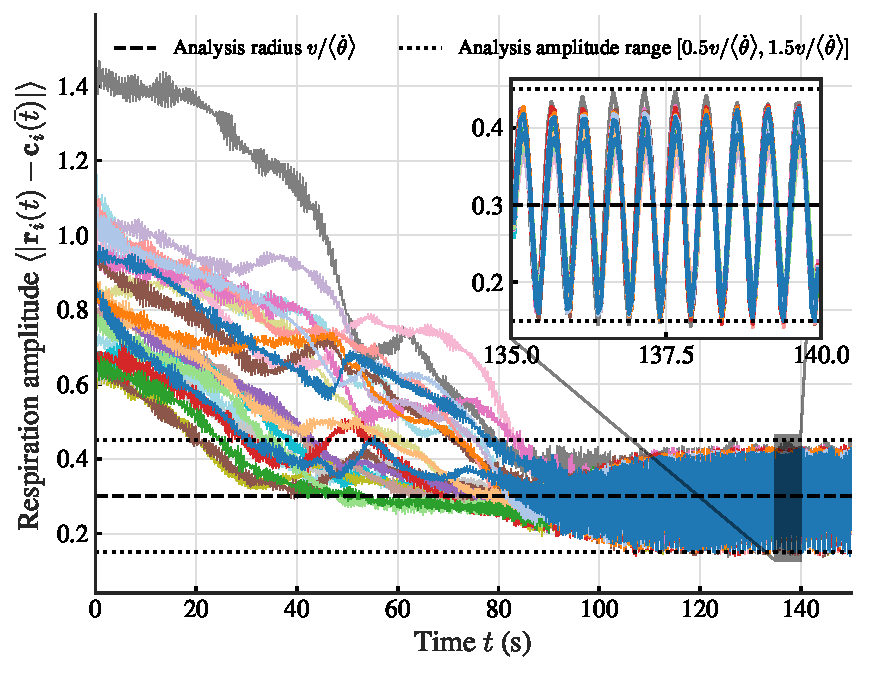
\includegraphics[width=0.8\textwidth]{./figs/respiration_amplitude_inset.pdf}
    \caption{
        \label{fig:respiration_amplitude}
        respiration amplitude of the system. 
        Different colors represent different cells, and the amplitude is defined as the distance between particles and the center of mass of the cell at final state ($\bar{t}=40$).
    }
\end{figure}

\begin{figure}[H]
        \centering
        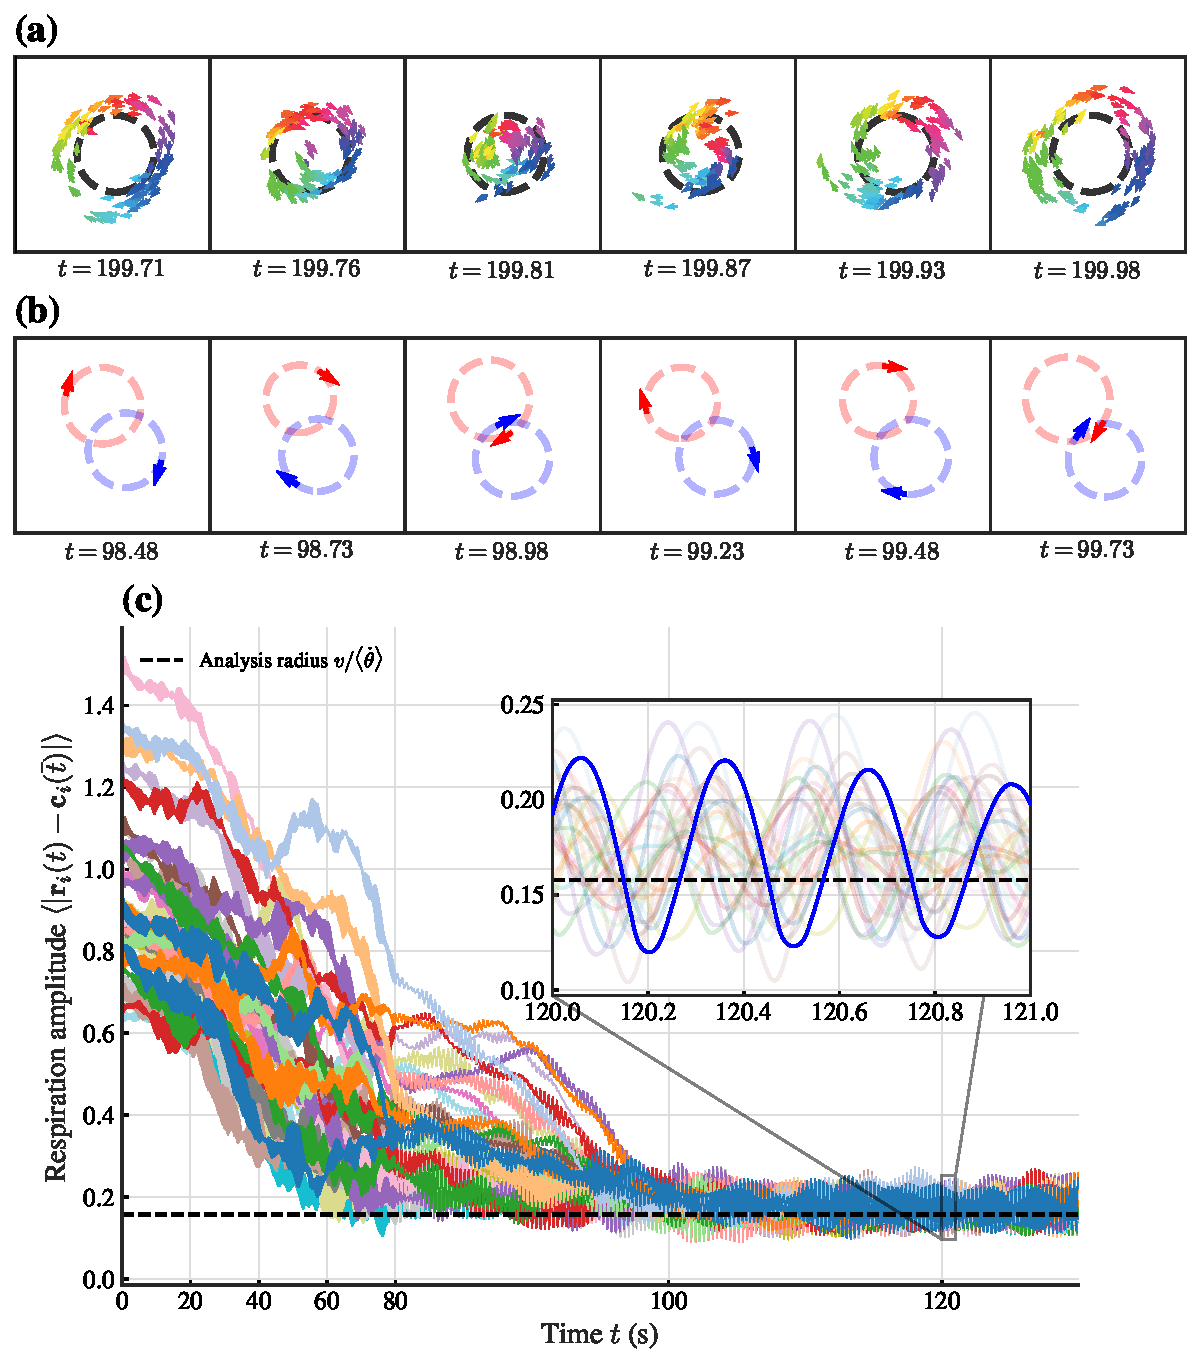
\includegraphics[width=0.8\textwidth]{./figs/respiration.pdf}
        \caption{
            \label{fig:respiration}
            (a, b) Respiration dynamics of vortex (a, $\alpha=0.6\pi$) and double clustered (b, $\alpha=0.9\pi$) unit cell. 
            In (a), dashed circle indicates vortex cell volume. In (b), red/blue arrows show phase-divided clusters; dashed circles show estimated trajectories.
            (c) Respiration amplitude over time for $\alpha=0.6\pi$.
        }
\end{figure}

\bibliography{ref}

\end{document}